Snapshotting is een vorm van versioning en is een on-site backup. Een bestandssysteem werkt met pointers naar de data. Een snapshot maakt nieuwe pointers naar de bestaande data. De data op het bestandssysteem en de data op de snapshot verwijzen dus naar dezelfde data, beide zijn gelijk. Als een bestand gewijzigd wordt dan verandert op het bestandssysteem de pointer naar de nieuwe data, terwijl de pointer vanuit de snapshot blijft staan naar de oude data. Zie figuur \ref{fig:snapshot} voor een grafische weergave van de werking van snapshots.

\begin{figure}[h]
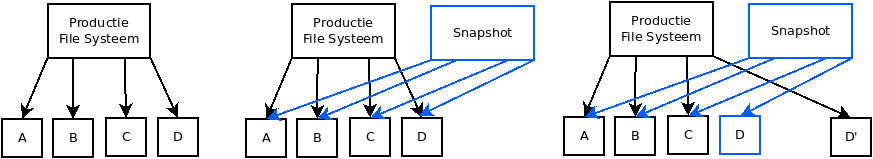
\includegraphics[width=\textwidth]{snapshot}
\centering
	\caption{Hoe snapshotting werkt}
	\label{fig:snapshot}
\end{figure}
Zo kunnen we met een minimale overhead terug naar een oude versie van onze data, welliswaar tegen de kosten van extra data gebruik op ons systeem.

